\documentclass[tikz,border=10pt]{standalone}
% Scale s = 0.009963 cm/px, origin at image centre (457.5, 319)
\usetikzlibrary{calc}
\begin{document}
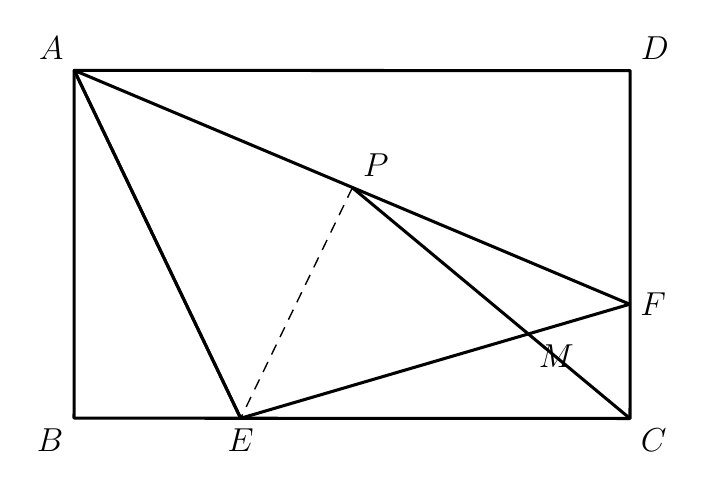
\begin{tikzpicture}[line join=round, line width=1.1pt,
  lbl/.style={font=\fontsize{11.5}{13.8}\selectfont}]
  % Vertices
  \coordinate (A) at (-3.5286233092944546,2.2062303048666534);
  \coordinate (D) at (3.532446301440139,2.2019505580444125);
  \coordinate (C) at (3.5297690261480676,-2.2152329786176135);
  \coordinate (B) at (-3.531300584586683,-2.210953231795362);
  \coordinate (E) at (-1.4149760815474979,-2.2126361684780007);
  \coordinate (F) at (3.526143163023008,-0.7640489348769468);
  \coordinate (P) at (0.0039737413089111495,0.71579122044823);
  % Intersection of EF and PC (label M)
  \coordinate (X) at (2.2355677435085095,-1.1411007695913735);

  % Quadrilateral sides
  \draw (A) -- (D) -- (C) -- (B) -- cycle;

  % Interior segments
  \draw (A) -- (F) -- (E) -- cycle;
  \draw (A) -- (E);
  % C-P ends at P (no overhang)
  \draw (C) -- (P);
  % Dashed P-E: dashes (not round dots), thin line
  \draw[line width=0.5pt, dash pattern=on 4pt off 3pt] (P) -- (E);

  % Labels
  \node[above left, lbl] at (A) {$A$};
  \node[above right, lbl] at (D) {$D$};
  \node[below left, lbl] at (B) {$B$};
  \node[below right, lbl] at (C) {$C$};
  \node[below, lbl] at (E) {$E$};
  \node[right, lbl] at (F) {$F$};
  \node[above right, lbl] at (P) {$P$};
  \node[below right, lbl] at (X) {$M$};
\end{tikzpicture}
\end{document}